\documentclass[10pt, a4paper]{article}
\usepackage[paper=a4paper, left=1.5cm, right=1.5cm, bottom=1.5cm, top=2cm]{geometry}
\usepackage[utf8]{inputenc}
\usepackage[T1]{fontenc}
\usepackage[spanish]{babel}
\usepackage{indentfirst}
\usepackage{fancyhdr}
\usepackage{lastpage}
\usepackage{calc}
\usepackage{caratula}
\usepackage{marvosym} % para \Faxmachine !
\usepackage{graphicx}
\usepackage{float}
% \PassOptionsToPackage{noend}{algpseudocode}% comment out if want end's to show
\usepackage{algpseudocode}
\usepackage{algorithm}
\usepackage{multicol}
\usepackage[hidelinks]{hyperref}
\graphicspath{{imagenes/}}
%\sloppy
\parskip=5pt % 10pt es el tamano de fuente

\usepackage{stringenc}
\usepackage{pdfescape}
\usepackage{color}
\definecolor{red}{RGB}{255,0,0}
\definecolor{blue}{RGB}{0,0,255}
\usepackage{amsmath}
\usepackage[makeroom]{cancel}
\usepackage{wrapfig}
\usepackage[font=small,labelfont=bf]{caption}


%% -------------------------
\errorcontextlines\maxdimen

% begin vertical rule patch for algorithmicx (http://tex.stackexchange.com/questions/144840/vertical-loop-block-lines-in-algorithmicx-with-noend-option)
\makeatletter
% start with some helper code
% This is the vertical rule that is inserted
    \newcommand*{\algrule}[1][\algorithmicindent]{\makebox[#1][l]{\hspace*{.5em}\thealgruleextra\vrule height \thealgruleheight depth \thealgruledepth}}%
% its height and depth need to be adjustable
\newcommand*{\thealgruleextra}{}
\newcommand*{\thealgruleheight}{.75\baselineskip}
\newcommand*{\thealgruledepth}{.25\baselineskip}

\newcount\ALG@printindent@tempcnta
\def\ALG@printindent{%
    \ifnum \theALG@nested>0% is there anything to print
        \ifx\ALG@text\ALG@x@notext% is this an end group without any text?
            % do nothing
        \else
            \unskip
            \addvspace{-1pt}% FUDGE to make the rules line up
            % draw a rule for each indent level
            \ALG@printindent@tempcnta=1
            \loop
                \algrule[\csname ALG@ind@\the\ALG@printindent@tempcnta\endcsname]%
                \advance \ALG@printindent@tempcnta 1
            \ifnum \ALG@printindent@tempcnta<\numexpr\theALG@nested+1\relax% can't do <=, so add one to RHS and use < instead
            \repeat
        \fi
    \fi
    }%
\usepackage{etoolbox}
% the following line injects our new indent handling code in place of the default spacing
\patchcmd{\ALG@doentity}{\noindent\hskip\ALG@tlm}{\ALG@printindent}{}{\errmessage{failed to patch}}
\makeatother

% the required height and depth are set by measuring the content to be shown
% this means that the content is processed twice
\newbox\statebox
\newcommand{\myState}[1]{%
    \setbox\statebox=\vbox{#1}%
    \edef\thealgruleheight{\dimexpr \the\ht\statebox+1pt\relax}%
    \edef\thealgruledepth{\dimexpr \the\dp\statebox+1pt\relax}%
    \ifdim\thealgruleheight<.75\baselineskip
        \def\thealgruleheight{\dimexpr .75\baselineskip+1pt\relax}%
    \fi
    \ifdim\thealgruledepth<.25\baselineskip
        \def\thealgruledepth{\dimexpr .25\baselineskip+1pt\relax}%
    \fi
    %\showboxdepth=100
    %\showboxbreadth=100
    %\showbox\statebox
    \State #1%
    %\State \usebox\statebox
    %\State \unvbox\statebox
    %reset in case the next command is not wrapped in \myState
    \def\thealgruleheight{\dimexpr .75\baselineskip+1pt\relax}%
    \def\thealgruledepth{\dimexpr .25\baselineskip+1pt\relax}%
}
% end vertical rule patch for algorithmicx
%%--------------------------



\begin{document}
\title{TDC -TP1}
\materia{Teoría de las Comunicaciones}
\submateria{Segundo cuatrimestre 2017}
\titulo{Informe}
\begin{center}
    
\includegraphics[width=0.7\textwidth]{caratula.jpg}
\end{center}
\subtitulo{TP1}
\integrante{Alejandro Ferrante}{371/09}{}
\integrante{Gonzalo Guillamon}{97/12}{}
\integrante{Malena Ivnisky}{421/12}{malenaivnisky@gmail.com}

\maketitle

\newpage\null\thispagestyle{empty}

\newpage
\thispagestyle{empty}
\setcounter{tocdepth}{3}
\tableofcontents

\newpage\null\thispagestyle{empty}

\newpage
\setcounter{page}{1}


%\includegraphics[width=\textwidth]{cookies}  ejemplo para incluir imagenes


\section{Introducción}

El objetivo de este trabajo práctico es analizar distintas capturas de red usando las herramientas vistas en la materia.


\section{Justificación de la elección de la fuente S2}

El objetivo de la fuente S2 es poder distinguir a los hosts de cada red, usando las IP dentro de los paquetes ARP capturados. Propusimos un modelo en el cual los símbolos son las IPs de los emisores de paquetes ARP del tipo who-has. Esto nos permite distinguir entre hosts comunes y routers, ya que esperamos que los routers envíen muchos más requests de ARP que el resto de los dispositivos conectados.

Elegimos el request de ARP y no el reply porque consideramos que este nos brindaría la misma información pero en menor cantidad (porque se envía en modo unicast). En este caso la dirección que nos importaría sería la de destino, la cual la mayoría de las veces pertenecería a routers.

%% me parece que esto esta horrible
\section{Experimento 1: Red de Starbucks}

\subsection{Descripción del contexto}

El experimento fue realizado en una red de FibertelZone, por medio de una conexión Wi-Fi en un local de Starbucks de Corrientes y Malabia. Dentro de la red se encuentran conectadas aproximadamente 10 notebooks y muchos celulares, además del router. La fecha de captura es Domingo 9 de Octubre de 2017.

\subsection{Descripción de la captura}

Capturamos 12000 paquetes. En la figura~\ref{protocolos1} se muestra la distribución de los protocolos en la red. Observamos que la mayoría de los paquetes son de tipo IPv4, otros son de tipo \texttt{0x86dd} (IPv6) y la minoría son de ARP.

Los paquetes de tipo IPv4 e IPv6 usan distintas versiones del protocolo IP. Los paquetes de tipo ARP son los usados por los hosts de una red para obtener direcciones MAC de otros dispositivos, a partir de su IP.

Esto es consistente, ya que la mayoría de los dispositivos usan IPv4/IPv6 para conectarse a Internet, y el porcentaje de paquetes ARP es considerable al haber muchos dispositivos conectados al mismo tiempo.

%% distribucion de protocolos (grafico)
\begin{figure}[H]
\centering
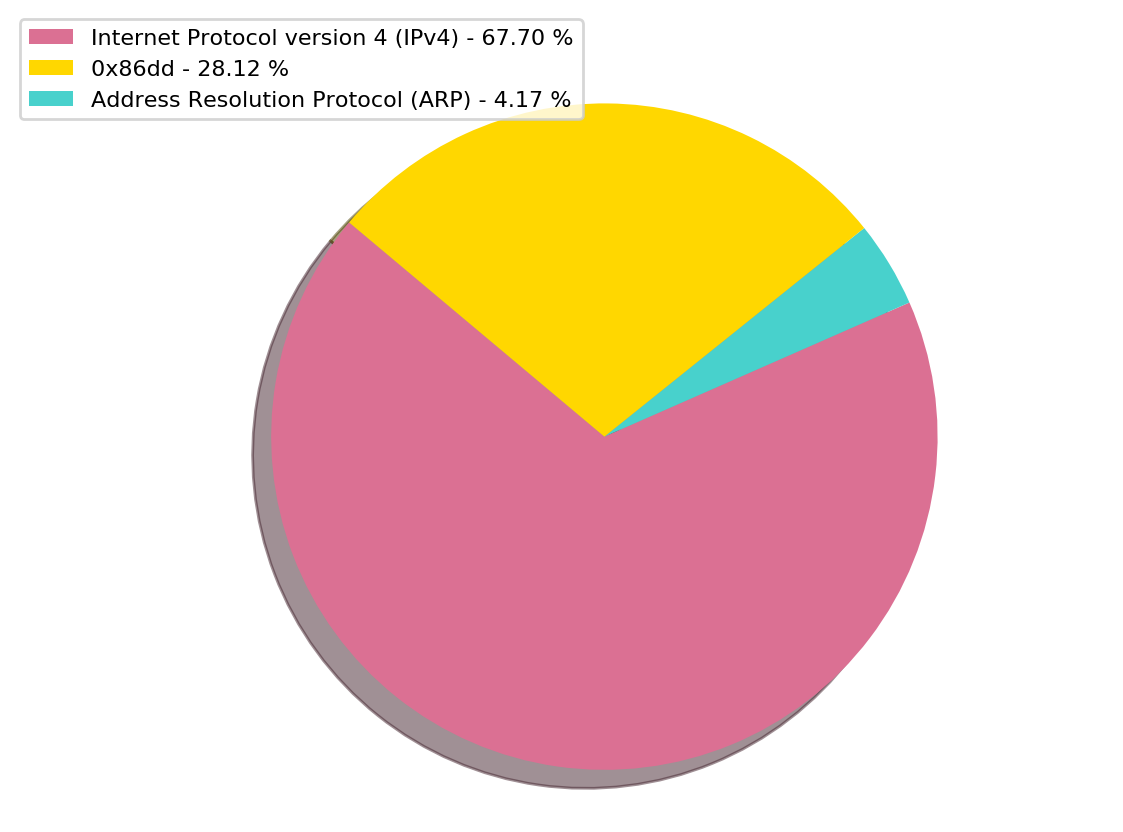
\includegraphics[width=0.7\textwidth]{protocolosRed1.png}
\caption{Gráfico que muestra la distribución de protocolos en la red.}
\label{protocolos1}
\end{figure}

En la figura~\ref{broadcast1} podemos ver el porcentaje de paquetes broadcast comparado con el total de paquetes. Vemos que esto representa un 16\% del total. En la figura~\ref{entropias1_1} vemos que los protocolos que aparecen en los paquetes de broadcast son ARP e IPv4. En cuanto a ARP, estos paquetes son los del tipo who-is, que mediante broadcast llegan al nodo cuya IP busca el emisor. 

%%% Y QUE PASA CON IPV4 BROADCAST?

\begin{figure}[H]
\centering
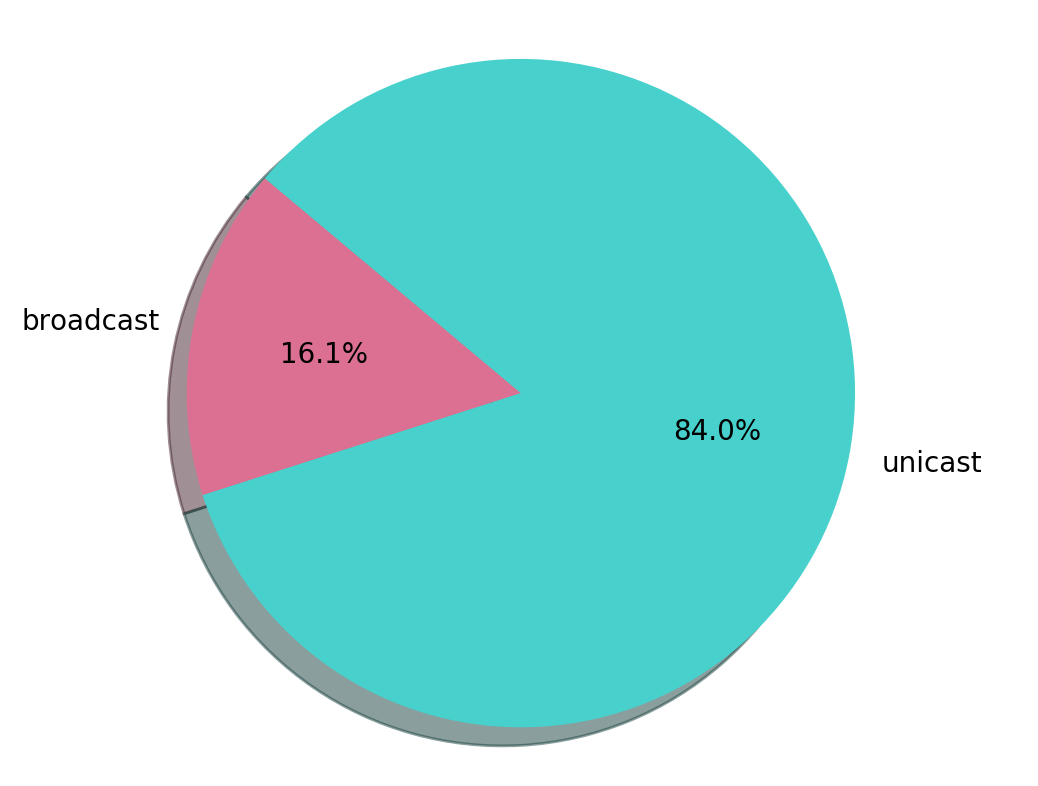
\includegraphics[width=0.7\textwidth]{broadcastRed1.png}
\caption{Gráfico que muestra los porcentajes de tráfico broadcast y unicast.}
\label{broadcast1}
\end{figure}

\subsection{Análisis de la captura}

Realizamos el modelado de la fuente $S_1$ según el enunciado. En la figura~\ref{entropias1_1} se encuentra el gráfico de la información de cada símbolo. Cuanta más información tenga un símbolo, quiere decir que es menos probable que aparezca. En esta red particular el símbolo con más información es representado por los paquetes unicast de tipo ARP. Estos paquetes son los is-at, las respuestas a los who-has. Tiene sentido ya que mientras que el request de ARP se hace mediante broadcast (o sea, mandando muchos paquetes), el reply es unicast (menos paquetes).

Además vemos que la entropía muestral es más de la mitad de la entropía máxima, esto es así porque la información de los distintos símbolos es comparable. El símbolo con más información (ARP, unicast) tiene aproximadamente 10 veces la información del menor (IPv4, unicast). La entropía máxima se alcanzaría si la información de todos los símbolos fuese la misma.

\begin{figure}[H]
\centering
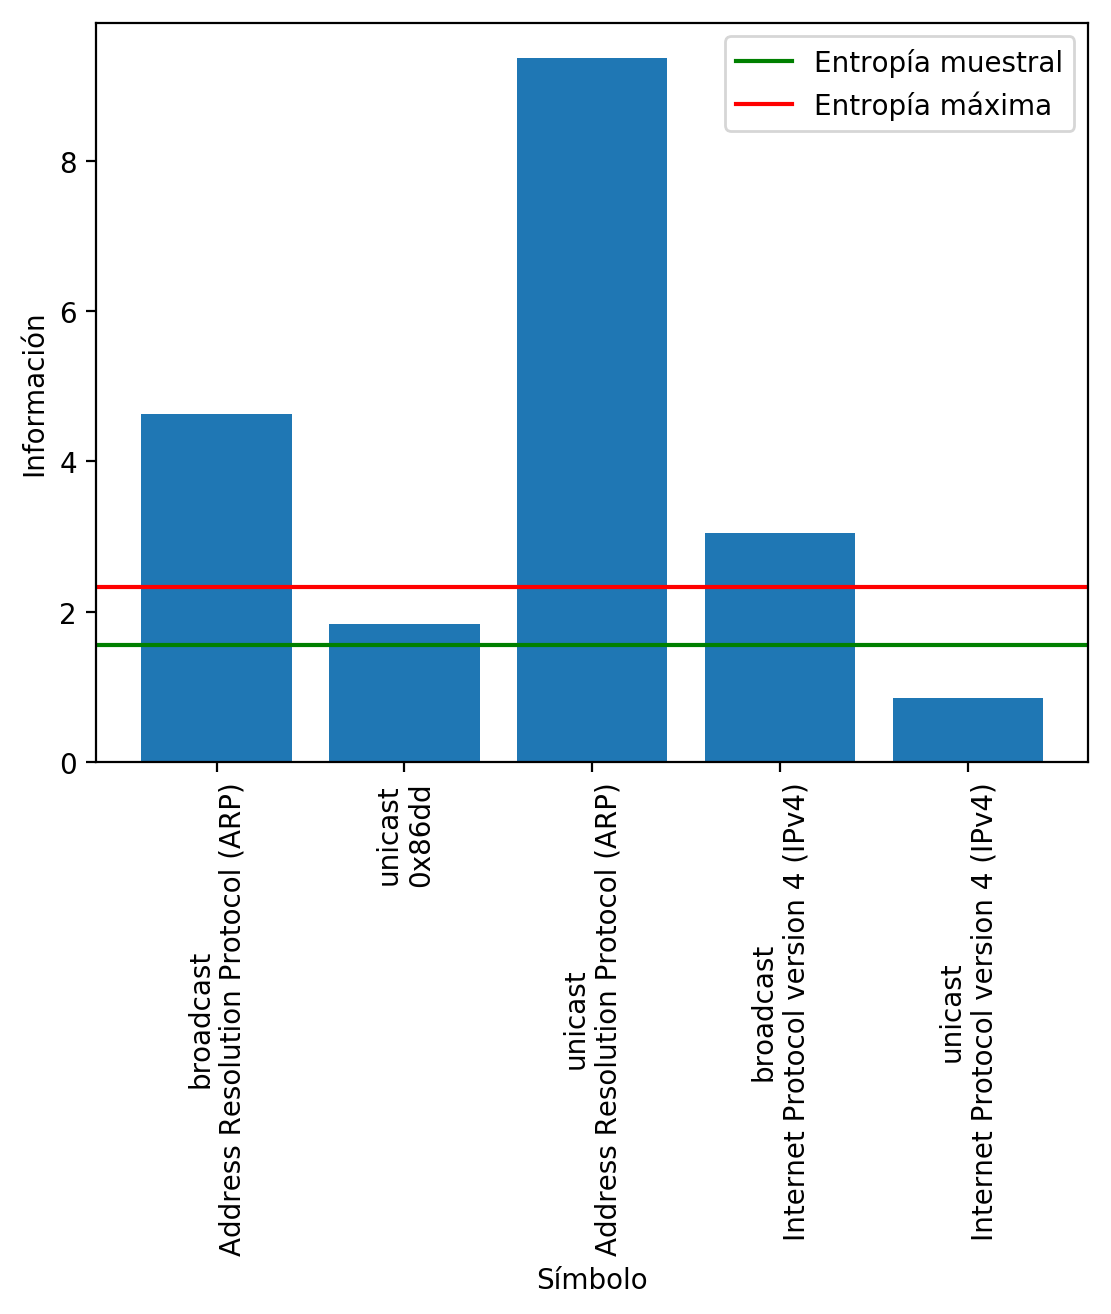
\includegraphics[width=0.7\textwidth]{entropiaS1Red1.png}
\caption{Gráfico de la información de los símbolos de la fuente $S_1$ observados en esta red. Se muestra la entropía muestral de $S_1$ y su entropía máxima.}
\label{entropias1_1}
\end{figure}

El análisis usando el modelado de la fuente $S_2$ (explicado anteriormente) se puede ver en la figura~\ref{entropias2_1}. En este caso vemos que los símbolos de la fuente podrían dividirse en 2 o 3 grupos de acuerdo a su información. Se observan algunos puntos distinguidos, en particular las 8 IPs con información menor a la entropía de $S_2$. Estas son las IPs que más requests de ARP hicieron. 

La entropía muestral es aproximadamente $\frac{4}{5}$ de la máxima. Es alta ya que hay muchos símbolos con valores parecidos de información; la máxima se alcanzaría con equiprobabilidad.

\begin{figure}[H]
\centering
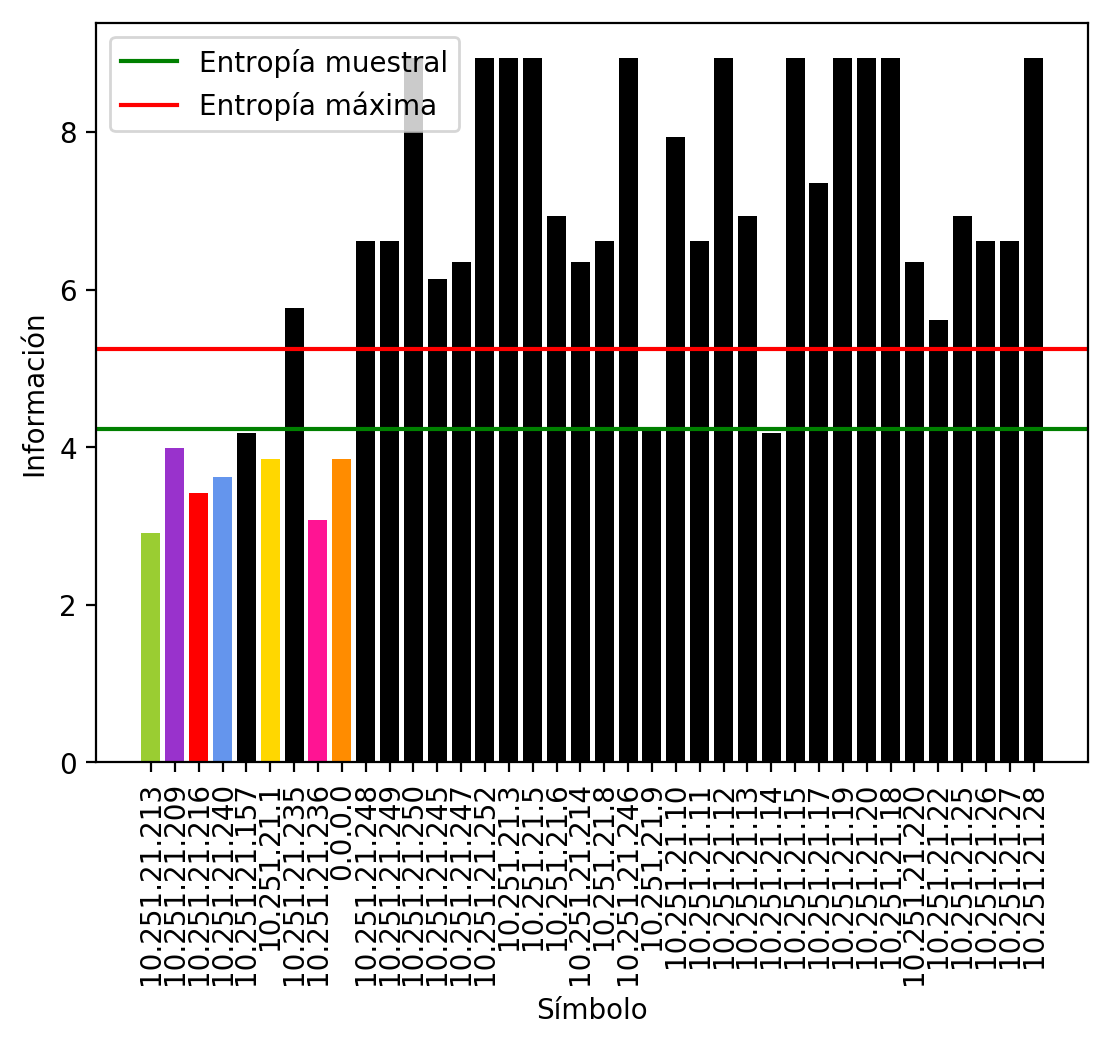
\includegraphics[width=0.7\textwidth]{entropiaS2Red1.png}
\caption{Gráfico de la información de los símbolos de la fuente $S_2$ observados en esta red. Se muestra la entropía muestral de $S_2$ y su entropía máxima.}
\label{entropias2_1}
\end{figure}

Por último graficamos la red subyacente de mensajes ARP, en la figura~\ref{grafo1}. Cada nodo del grafo representa una IP interviniente en al menos un mensaje ARP de la red, y cada eje orientado representa que la primera IP envió al menos un mensaje a la segunda. No estamos distinguiendo entre paquetes de tipo who-has o is-at. Podemos ver que el nodo central se comunica separadamente con muchos otros nodos, por lo que creemos que es el router del Stabucks.

\begin{figure}[H]
\centering
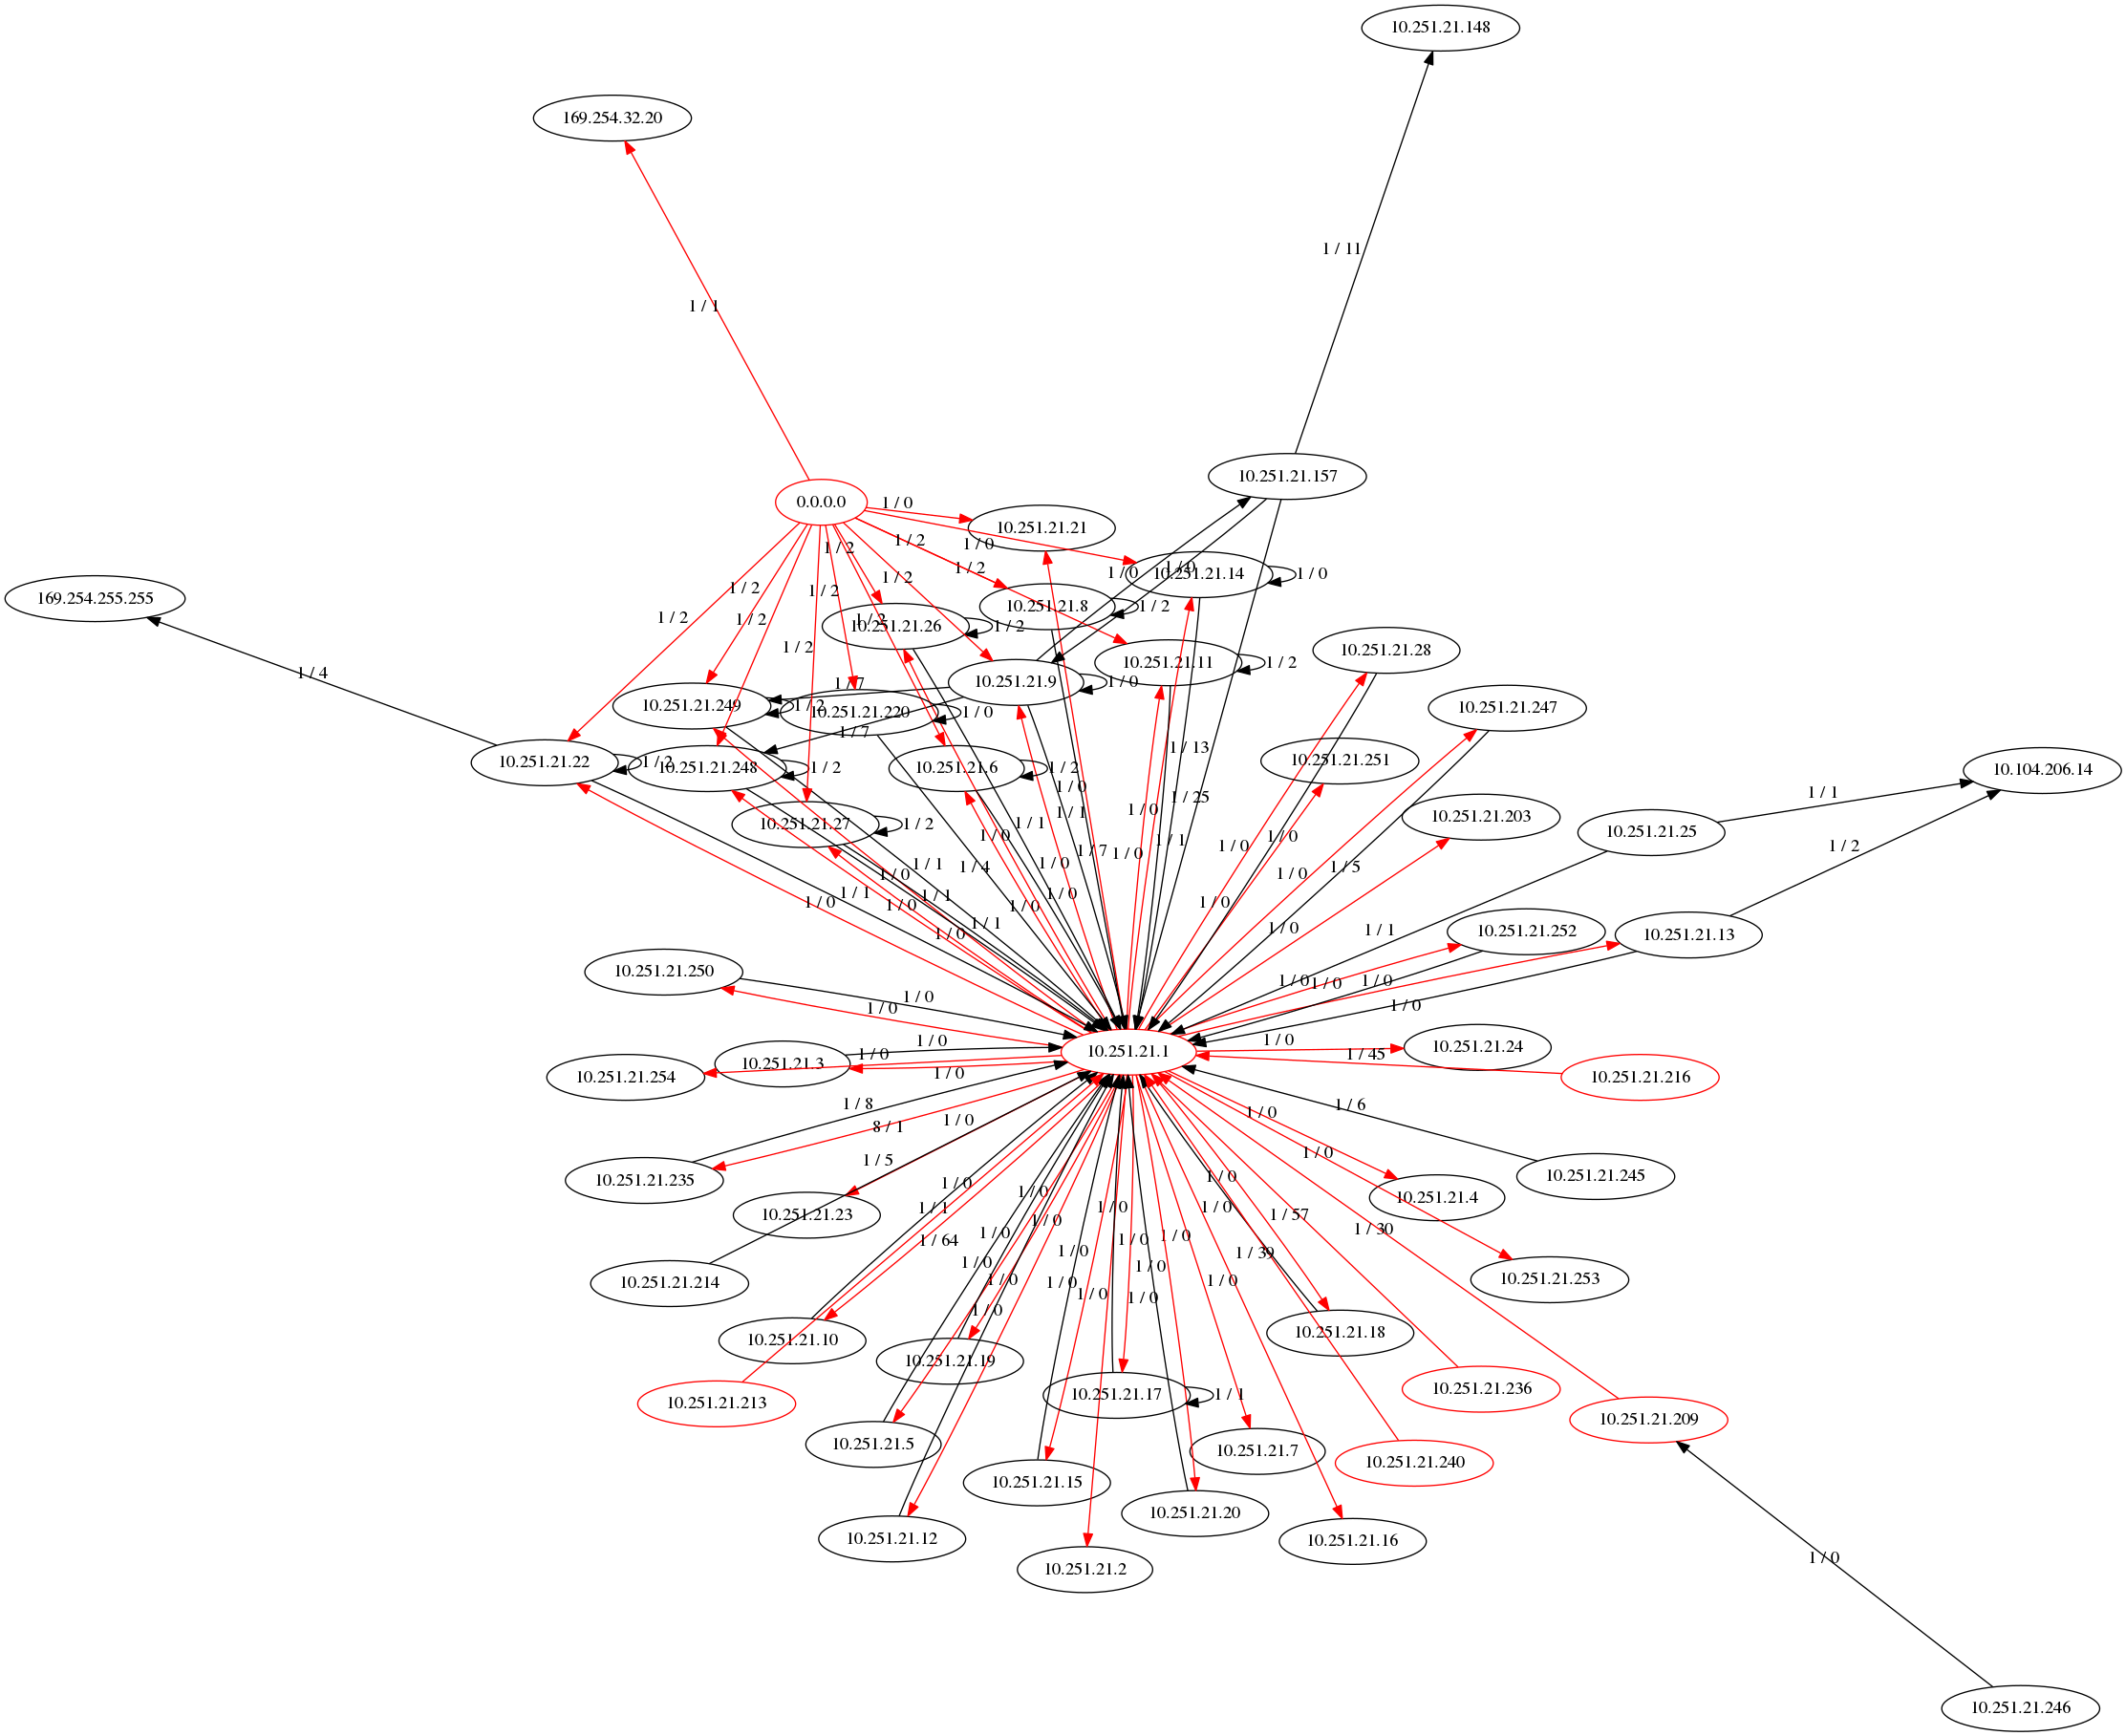
\includegraphics[width=\textwidth]{grafoRed1.png}
\caption{Grafo de la red de mensajes ARP subyacente.}
\label{grafo1}
\end{figure}

\section{exp2}
\section{Experimento 3: Red hogareña cableada}

\subsection{Descripción del contexto}

\subsection{Descripción de la captura}

\subsection{Análisis de la captura}

\section{Conclusiones}

No vimos falsos negativos. En general hay outliers de más, no de menos. 

Este método no es muy efectivo porque las velocidades de internet en cada país no son las mismas, y eso no es tenido en cuenta.

Además, el hecho de que en cada envío los paquetes puedan tomar una ruta diferente hace que los experimentos devuelvan resultados con muchos outliers y datos inconsistentes.

Por otra parte, el analisis de las IPs visitadas era razonable, aunque el camino elegido no siempre fuera el más ``intuitivo''. Sin embargo, varios de los resultados que obtuvimos nos llevan a la conclusión de que tampoco son datos certeros.

\end{document}
